\documentclass[CS4204-Notes.tex]{subfiles}
\begin{document}

\section{Locks and lock-free}
In programming with locks, we want to be explicit about goals and trade-offs. A benefit in one dimension often has costs in another. For example an increase in performance that prevents a data structure from being used in some particular setting. The ultimate goal is to increase performance, either as time or resources used. The trade-off is generally if an implementation can scale well enough to out-perform a good sequential implementation.
\n
There are three kinds of parallel hardware
\begin{enumerate}
\item Multi-threaded cores - increase utilisation of a core or memory bandwidth. Long latency oeprations are tolerated and the peak operations per core (ops/core) is fixed.
\item Multiple cores - increase operations per core (ops/core). However caches and off-chip resources don't always cale proportionately
\item Mult-processor machines - increase operations per core and often \textit{do} scale cache and memory capacities and bandwidth proportionately. Has NUMA (non-uniform memory access) memory effects.
\end{enumerate}

\subsection{Locks}
Locks are the basic building block for concurrency control. It provides a guarantee that other threads do not interfere with the current thread if the lock is being held. In a shared-memory system, threads can \textit{always} interfere, so locks must be strict. Different languages have their own implementations of locks
\begin{itemize}
\item C \texttt{pthread_mutex}
\item Java \texttt{synchronized} blocks
\item Haskell \texttt{MVar}
\end{itemize}
The locks themselves are typically implemented with lower-level operations such as Test-and-Set (TAS) and Compare-and-Swap(CAS). Furthermore, assembly languages have specific instructions that can be used for atomic lock operations, such as \texttt{lock xchg} in x86 and \texttt{ldrex}/\texttt{strex} in ARM.

\subsubsection{Comapre and swap}
The compare and swap operation is used to implement both concurrency primitives like semaphores/mutexes, as well as more sophisticated lock-free and wait-free algorithms.
\n
The idea behind compare and swap is to read some memory location and remember the old value. Based on that old value, a new value is computed. A thread then tries to swap in the new value using CAS, where the comparison checks the location still being equal to the old value. If the CAS fails, it has to be repeated.
\begin{lstlisting}[caption={Compare and swap},language=C]
  int compareAndSwap(int *b, int exp, int place)
  {
    // b is a pointer to the locatio we think contains exp
    
    int result;

    atomic
    {
      // read current value of location b
      result = *b;

      // update b only if we guessed right
      if (result == exp) *b = place;
    }
    return result;
  }
  
\end{lstlisting}

\subsubsection{Test and set}
Test and set is an instruction used to write (set) a memory location and return its old value as a single atomic operation. If multiple processes access the same memory location, and if a process is currently performing a test-and-set, no other process may begin another test-and-set until the first process's test-and-set is finished. 
\begin{lstlisting}[caption={Test and set},language=C]
  bool testAndSet(bool *b)
  {
    // b is a location holding true or false
    
    bool result;

    atomic
    {
      // read current value of location b
      result = *b;

      // atomically set it to TRUE
      *b = TRUE;
    }
    return result;
  }
\end{lstlisting}
If two or more threads try to \texttt{testAndSet} at once, only one return \texttt{FALSE}, the rest return \texttt{TRUE}. The lock is initialisation to \texttt{FALSE}, which means the lock is available.
\begin{lstlisting}[caption={Implementing a lock with test and set}, language=C]
  void acquireLock(bool *lock)
  {
    while (testAndSet(lock))
    {
      // do nothing
    }
  }

  void releaseLock(bool *lock)
  {
    *lock = FALSE;
  }
  
\end{lstlisting}
Each call tries to acqurie the lock, returning \texttt{TRUE} if it is already held.

\subsubsection{Issue with locks}
Using a test-and-set implementation of locks causes contention on the lock variable, as each thread spins in a while loop. Furthermore, each thread has to atomically set the lock variable on each call, which must be done sequentially to ensure atomicity. The spinning on the while loop is also a waste of system resources as they are wasted clock cycles.
\n
The general problem is that there is no logical conflict between two failed lock acquires while a physical conflict in the cache does occur. For a good algorithm, we wish to only introduce physical conflicts if a logical conflict occurs. For example
\begin{itemize}
\item Successful lock-acquire and failed lock-acquire at the same time
\item Successful value insertion and failed value insertion at the same time
\end{itemize}
We do not want to introduce physical conflicts in cases of two failed lock acquires, or two successful insertions. A fix to this issue would be to spin when the lock is held, rather than spin trying to acquire the lock all the time
\begin{lstlisting}[caption={Spin while the lock is held to reduce contention}, language=C]
  void acquireLock(bool *lock)
  {
    do
    {
      while (*lock);
    } while (testAndSet(lock));
  }
\end{lstlisting}
By spinning while the lock is held and only trying to test and set when it is free, contention is reduced, making it significantly more scalable to more threads. However, this leads to another problem of stampedes. Once the lock is freed, all the threads waiting for it try to access it at the same time, again causing contention at that particular moment. To alleivate this issue, \textbf{backoff} algorithms can be used.
\n
By using back-offs, each threads starts spinning and watches the lock for $c$ iterations. If the lock does not become free, the threads spin locally for $s$ iterations without watching the lock. Setting different values for $c$ and $s$ will have a different effect on the efficiency and concurrency of the program.
\n
Lower value of $c$
\begin{itemize}
\item Less time to build up a set of threads that will stampede
\item Less contention in the memory system
\item Risk of a delay in noticing when the lock becomes free when no thread is watching
\end{itemize}
\vspace{\baselineskip}
Higher values of $c$
\begin{itemize}
\item Less likelihood of a delay between when a lock is released and a wating thread notices
\end{itemize}
\vspace{\baselineskip}
Lower value of $s$
\begin{itemize}
\item More responive to the lock becoming available
\end{itemize}
\vspace{\baselineskip}
\begin{itemize}
\item If the lock doesn't become available then the thread makes fewer accesses to the shared variable (less contention)
\end{itemize}
The rule of thumb with back-off heuristics is to generally spin for a duration that's comparable with the shortest back-off interval and exponentially increase the per-thread back-off interval, resetting it when the lock is acquired. Finally a maximum back-off interval should be used that is large enough that waiting threads don't interfere with the other threads' performance.

\subsection{Non-blocking algorithms}
To be able to scale to a large number of cores, we need critical sections to be rare and short. A lock implementation may involve updating a few memory locations, increasing the amount of critical sections needed. Using data structures may help reduce this to only specific memory locations. If we try to shrink critical sections then the time in the lock implementation becomes proportionately greater. So the idea moving forward is to try and make the cost of the operations in the critical section lower or try to write the critical sections correctly \textit{without} locks.
\n
These are known as non-blocking algorithms, in which failure or suspension of any thread \textit{cannot} cause failure or suspension of another thread. Traditional non-blocking algorithms are lock-free is there is guaranteed system-wide progress, and wait-free is there is guaranteed per-thread progress.

\subsubsection{Wait-freedom}
Wait-freedom is the strongest non-blocking guarantee of progress, combining system-wide throughput with starvation-freedom. An algorithm is defined as wait-free if every operation has a bound on the number of steps the algorithm will take before the operation completes. In other words, a thread will finish its own operations if it continues executing steps.
\begin{figure}[H]
  \centering
  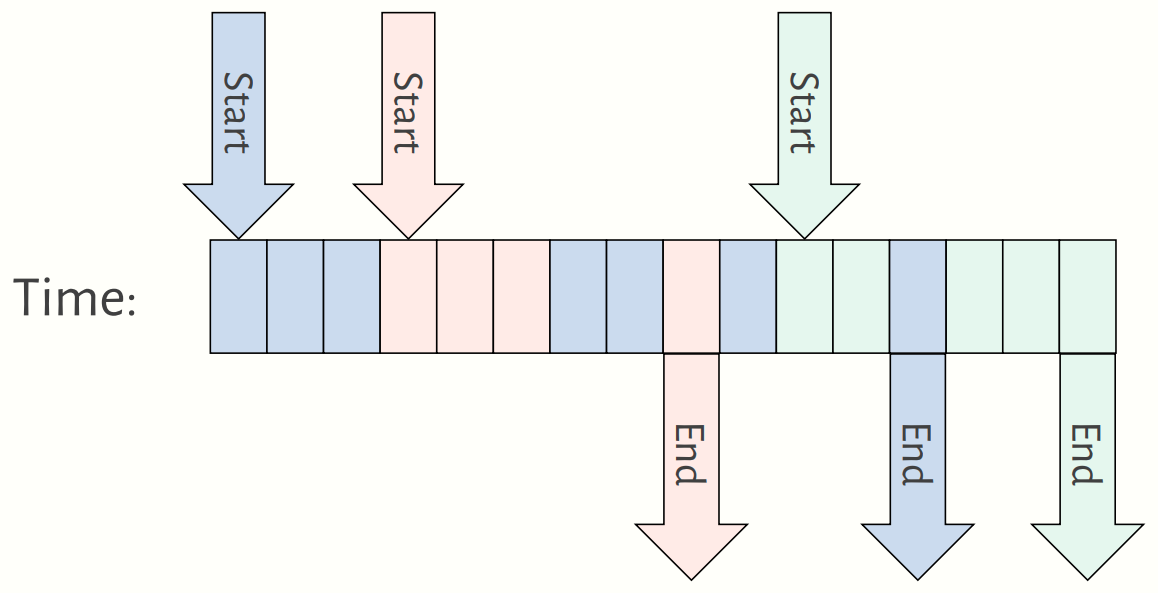
\includegraphics[width=0.8\textwidth, keepaspectratio]{imgs/wait-free.png}
\end{figure}
\noindent
General construction techniques for wait-free algorithms exist (called universal constructions) which uses CAS as a building block. However, their performance does not in general match even simple blocking designs. There are a few approaches that can be taken for wait-free algorithms:
\begin{itemize}
\item Queueing and helping strategies - everyone ensures the oldest operation makes progress. However, often a high sequential overhead and therefore has limited scalability
\item Fast-path/slow-path constructions - Start with a faster lock-free algorithm and switch over to a wait-free algorithm if there is no progress. If done carefully, we can obtain wait-free progress overall
\end{itemize}
In practice, progress guarantees can vary between operations on a shared object, for example using a wait-free find, then a lock-free delete.
\begin{lstlisting}[caption={Wait-free using atomic increment}, language=C]
  void inc (Object* o)
  {
    atomic_increment(o -> r);
  }

  void dec (Object* o)
  {
    if (0 == atomic_decrement(o -> r))
    {
      delete o;
    }
  }
  
\end{lstlisting}
This works because we defer the atomic operation to the hardware, which will likely use locks, but on this higher-level software, only a single atomic operation is needed, which guarantees wait-free progress.


\subsubsection{Lock-freedom}
Lock-freedom allows individual threads to starve, but guarantees system-wide throughout. An algorithm is lock-free if, when the program threads are run for a sufficiently long time, at least one of the threads makes progress. In other words, this means that some thread will finish its operation if all threads continue taking steps. All wait-free algorithms are lock-free.
\begin{figure}[H]
  \centering
  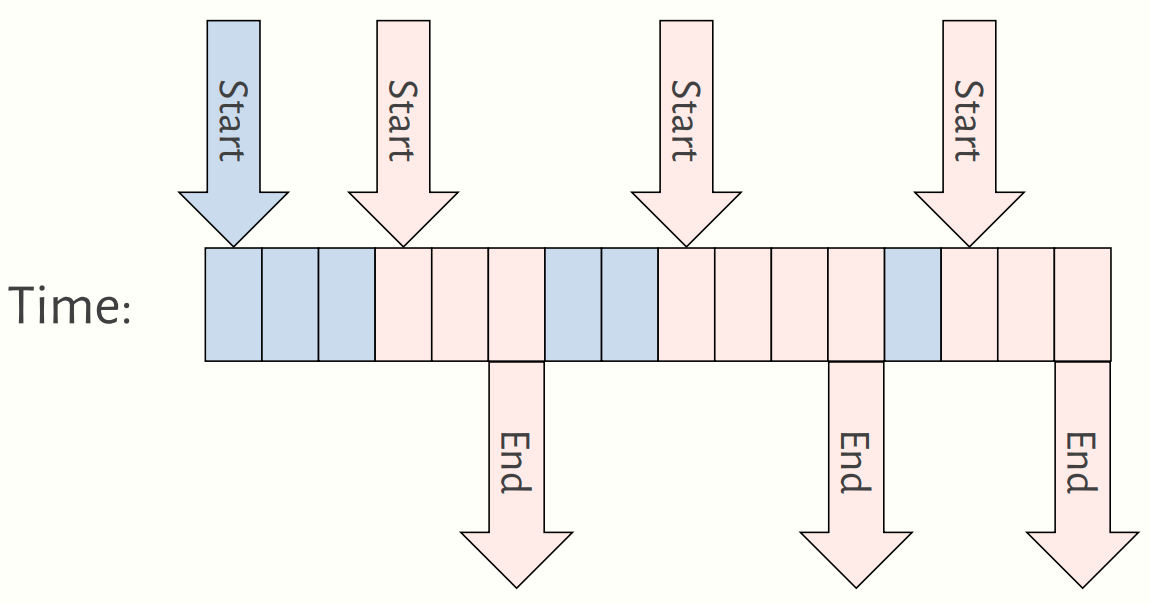
\includegraphics[width=0.8\textwidth, keepaspectratio]{imgs/lock-free.png}
\end{figure}
\noindent
Lock-free algorithms ensure that one thread only has to repeat work if some other thread has made \textit{real progress}, for example an insertion operation has to start again if it finds that a conflicting update has occurred. In particular, if one thread is suspended, then a lock-free algorithm guarantees that the remaining threads can still make progress, so there will be no deadlock where two threads contend for the same mutex lock. The difference between wait-free and lock-free is that wait-free operation by each process is guaranteed to succeed in a finite number of steps, regardless of the other processors.
\begin{lstlisting}[caption={Lock-free algorithm to increment a counter}, language=C]
  void inc(int counter)
  {
    int val = counter;
    while(!CAS(val, &counter, val+1))
    {
      val = counter;
    }
  }
\end{lstlisting}
This is not wait-free, as there is no guarantee that any particular thread will succeed. However, it is also not locking, because there is no critical section where one thread could block and prevent any other thread from accessing a shared lock.

\subsubsection{Obstruction-freedom}
Obstruction-freedom is the weakest natural non-blocking progress guarantee. An algorithm is obstruction-free if at any point, a single thread executed in isolation for a bounded number of steps will complete its operation. In other words, a thread will finish its own operation if it runs in isolation. All lock-free algorithms are obstruction-free.
\begin{figure}[H]
  \centering
  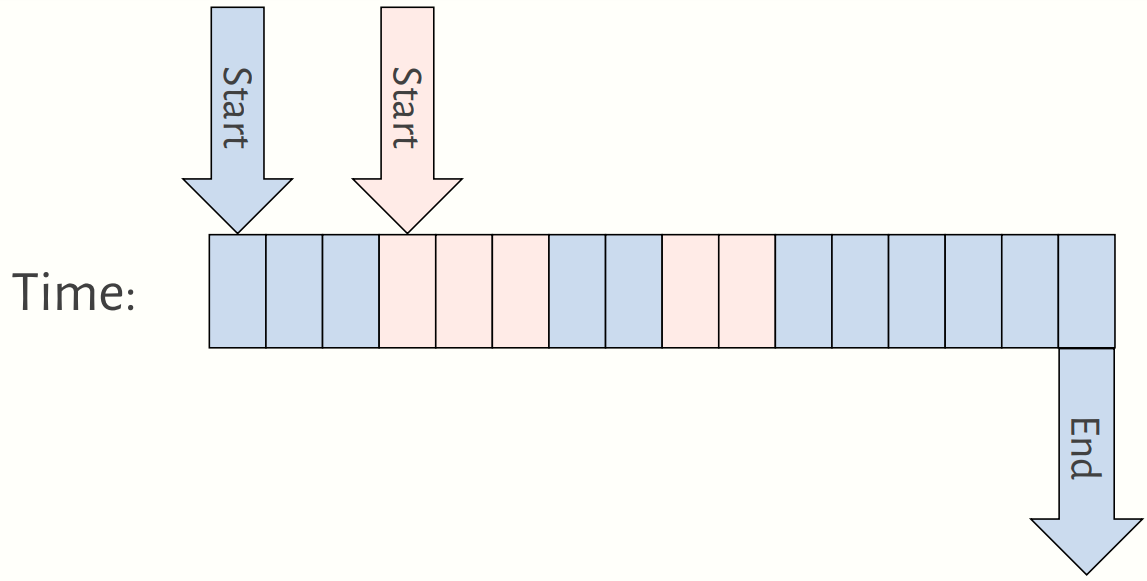
\includegraphics[width=0.8\textwidth, keepaspectratio]{imgs/obstruction-free.png}
\end{figure}
\noindent
Obstruction-free algorithms only ensure that none of the low-level steps leave a data structure broken. It does this by demanding that any partially completed operation can be aborted and the changes made rolled back. A \textbf{contention manager} is used to reduce the likelihood of live-lock.
\begin{lstlisting}[caption={Obstruction-free algorithm to increment a counter}, language=C]
  void inc(int counter)
  {
    while (true)
    {
      int val = LL(counter); //LL - weak load-linked
      if (SC(counter, val+1)) //SC - store-conditional
      {
        return;
      }
    }
  }

\end{lstlisting}
Because this algorithm requires two atomic steps (LL then SC), the LL operation on one thread will prevent an SC on another thread from succeeding.

\subsection{The ABA problem}
The ABA problem is a problem that occurs when memory deallocation and reclamation happens. THe main issue is when a location is read twice, has the same value for both reads where the fact that the \textit{value is the same} is used to indicate that nothing has change. However, another thread can execute between the two reads and change the value, do other work, then change the value back, thus fooling the first thread into thinking that nothing has changed, even though the work done by the second thread violates that assumption. The sequence of events is generally as follows:
\begin{itemize}
\item Process $P_{1}$ reads value A from shared memory
\item $P_{1}$ is pre-empted, allowing process $P_{2}$ to run
\item $P_{2}$ modifies the shared memory value A to value B and back to A before preemption
\item $P_{1}$ begins execution again, sees that the shared memory value has not changed and continues
\end{itemize}
Although $P_{1}$ can continue executing, it is possible that the behaviour will not be correct due to any hidden modifications in shared memory.
\n
A common case of the ABA problem is encountered when implementing a lock-free data structure. If an item is removed from the list, deleted and then a new item is allocated and added to the list, it is common for the allocated object to be at the same location as the deleted object. A pointer to the new item is therefore sometimes equal to a pointer to the old item even though the value has changes, which is an ABA problem.

\subsubsection{Solutions against the ABA problem}
\begin{itemize}
\item Add a tag/stamp to the pointer. For example, an algorithm using CAS on a pointer might use the low bits of the address to indicate how many times the pointer has been successfully modified. Because of this, the next CAS will fail even if the pointer addresses are the same because the tag bits will not match.
\item Extra guards during deallocation/reallocation
\item Hardware support
\end{itemize}

\end{document}